

\chapter{Classes and objects  |  类和对象}
\label{clobjects}

At this point you know how to use
functions to organize code and
built-in types to organize data.  The next step is to learn
``object-oriented programming'', which uses programmer-defined types
to organize both code and data.  Object-oriented programming is
a big topic; it will take a few chapters to get there.

目前你已经知道如何使用函数来组织你的代码,同时用内置的类型来管理数据。
下一步我们将学习 ``面向对象编程'',即使用
程序员定义的类来组织代码和数据。
面向对象编程是一个很大的话题,讲完需要一些章节。

\index{object-oriented programming}

Code examples from this chapter are available from
\url{http://thinkpython2.com/code/Point1.py}; solutions
to the exercises are available from
\url{http://thinkpython2.com/code/Point1_soln.py}.

本章的示例代码可以在\href{http://thinkpython2.com/code/Point1.py}{此处} 获取;
练习题的答案可以在\href{http://thinkpython2.com/code/Point1_soln.py}{此处} 获取。


\section{Programmer-defined types  |  程序员自定义类型}
\label{point}
\index{programmer-defined type}  \index{type!programmer-defined}

We have used many of Python's built-in types; now we are going
to define a new type.  As an example, we will create a type
called {\tt Point} that represents a point in two-dimensional
space.

我们已经使用过了许多 Python 的内置类型;
现在我们要定义一个新类型。 举个例子,我们来创建一个叫做 \li{Point} 的类型,代表二维空间中的一个点。

\index{point, mathematical}

In mathematical notation, points are often written in
parentheses with a comma separating the coordinates. For example,
$(0,0)$ represents the origin, and $(x,y)$ represents the
point $x$ units to the right and $y$ units up from the origin.

在数学记法中,点通常被写成在两个小括号中用一个逗号分隔坐标的形式。
例如 $(0,0)$ 代表原点,$(x,y)$ 代表原点向右 $x$ 个单位,向上 $y$ 个单位的点。

There are several ways we might represent points in Python:

在 Python 中,有几种表示点的方法:

\begin{itemize}

\item We could store the coordinates separately in two
variables, {\tt x} and {\tt y}.

\item 我们可以将坐标存储在两个独立的变量,\li{x} 和 \li{y} 中。

\item We could store the coordinates as elements in a list
or tuple.

\item 我们可以将坐标作为一个列表或者元组的元素存储。

\item We could create a new type to represent points as
objects.

\item 我们可以创建一个新类型将点表示为对象。

\end{itemize}
\index{representation}

Creating a new type
is more complicated than the other options, but
it has advantages that will be apparent soon.

创建一个新类型比其他方法更复杂,但是它的优势一会儿会显现出来。

A programmer-defined type is also called a {\bf class}.
A class definition looks like this:

程序员自定义类型 (A programmer-defined type) 也被称作 {\em 类} (class)。  像这样定义一个对象:

\index{class}  \index{object!class}
\index{class definition}  \index{definition!class}

\begin{lstlisting}
class Point:
    """Represents a point in 2-D space."""
\end{lstlisting}
%
The header indicates that the new class is called {\tt Point}.
The body is a docstring that explains what the class is for.
You can define variables and methods inside a class definition,
but we will get back to that later.

头部语句表明新类的名称是 \li{Point} 。
主体部分是文档字符串,用来解释这个类的用途。
你可以在一个类的定义中定义变量和函数,稍后会讨论这个。

\index{Point class}  \index{class!Point}  \index{docstring}

Defining a class named {\tt Point} creates a {\bf class object}.

定义一个叫做 \li{Point} 的类将创建了一个 {\em 类对象} (class object)。

\begin{lstlisting}
>>> Point
<class '__main__.Point'>
\end{lstlisting}
%
Because {\tt Point} is defined at the top level, its ``full
name'' is \verb"__main__.Point".

由于 \li{Point} 是定义在顶层的,所以它的``全名'' 是 \li{__main__.Point} 。

\index{object!class}  \index{class object}

The class object is like a factory for creating objects.  To create a
Point, you call {\tt Point} as if it were a function.

类对象就像是一个用来创建对象的工厂。
要创建一个点,你可以像调用函数那样调用 \li{Point} 。

\begin{lstlisting}
>>> blank = Point()
>>> blank
<__main__.Point object at 0xb7e9d3ac>
\end{lstlisting}
%
The return value is a reference to a Point object, which we
assign to {\tt blank}.

返回值是一个 \li{Point} 对象的引用,我们将它赋值给 \li{blank} 。

Creating a new object is called
{\bf instantiation}, and the object is an {\bf instance} of
the class.

创建一个新对象的过程叫做 {\em 实例化} (instantiation) ,这个新对象叫做这个类的一个 {\em 实例} (instance)。

\index{instance}  \index{instantiation}

When you print an instance, Python tells you what class it
belongs to and where it is stored in memory (the prefix
{\tt 0x} means that the following number is in hexadecimal).

当你试图打印一个实例,Python 会告诉你它属于哪个类,
以及它在内存中的存储地址(前缀 \li{0x} 代表紧跟后面的数是以十六进制表示的)。

\index{hexadecimal}

Every object is an instance of some class, so ``object'' and
``instance'' are interchangeable.  But in this chapter I use
``instance'' to indicate that I am talking about a programmer-defined
type.

每一个对象都是某种类的实例,所以``对象''和``实例''可以互换。  但是在这章我用 ``实例'' 来表示我在讨论程序员自定义类型。


\section{Attributes  |  属性}
\label{attributes}
\index{instance attribute}  \index{attribute!instance}
\index{dot notation}

You can assign values to an instance using dot notation:

你可以使用点标记法向一个实例进行赋值操作:

\begin{lstlisting}
>>> blank.x = 3.0
>>> blank.y = 4.0
\end{lstlisting}
%
This syntax is similar to the syntax for selecting a variable from a
module, such as {\tt math.pi} or {\tt string.whitespace}.  In this case,
though, we are assigning values to named elements of an object.
These elements are called {\bf attributes}.

这个语法类似于从一个模块中使用变量的语法,比如 \li{math.pi} 和 \li{string.whitespace} 。  不过在这个例子中,我们是给一个类中已命名的元素赋值。  这类元素叫做 {\em 属性} (attributes)。

As a noun, ``AT-trib-ute'' is pronounced with emphasis on the first
syllable, as opposed to ``a-TRIB-ute'', which is a verb.

作为名词的时候,``属性'' 的英文 ``AT-trib-ute'' 的重音在第一个音节上,作为动词的时候,``a-TRIB-ute'' 重音在第二个音节上。

The following diagram shows the result of these assignments.
A state diagram that shows an object and its attributes is
called an {\bf object diagram}; see Figure~\ref{fig.point}.

下面\hyperref[fig.point]{这张图}展示了这些赋值操作的结果。 说明一个对象及其属性的状态图叫做 {\em 对象图} (object diagram); 见图~\ref{fig.point}。

\index{state diagram}  \index{diagram!state}
\index{object diagram}  \index{diagram!object}

\begin{figure}
\centerline
{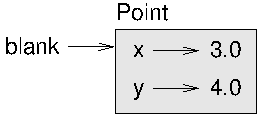
\includegraphics[scale=0.8]{../source/figs/point.pdf}}
\caption{Object diagram.}
\label{fig.point}
\end{figure}

The variable {\tt blank} refers to a Point object, which
contains two attributes.  Each attribute refers to a
floating-point number.

变量 \li{blank} 引用了一个 \li{Point} 类,这个类拥有了两个属性。
每个属性都引用了一个浮点数。

You can read the value of an attribute using the same syntax:

你可以使用相同的语法读取一个属性的值:

\begin{lstlisting}
>>> blank.y
4.0
>>> x = blank.x
>>> x
3.0
\end{lstlisting}
%
The expression {\tt blank.x} means, ``Go to the object {\tt blank}
refers to and get the value of {\tt x}.''  In the example, we assign that
value to a variable named {\tt x}.  There is no conflict between
the variable {\tt x} and the attribute {\tt x}.

表达式 \li{blank.x} 的意思是,``前往 \li{blank} 所引用的对象并且获取 \li{x} 的值''。
在这个例子中,我们将获取到的值赋值给了一个叫做 \li{x} 的变量。
变量 \li{x} 和属性 \li{x} 并不会冲突。

You can use dot notation as part of any expression.  For example:

你可以在任何表达式中使用点标记法。 例如:

\begin{lstlisting}
>>> '(%g, %g)' % (blank.x, blank.y)
'(3.0, 4.0)'
>>> distance = math.sqrt(blank.x**2 + blank.y**2)
>>> distance
5.0
\end{lstlisting}

%
You can pass an instance as an argument in the usual way.
For example:

你可以将一个实例作为参数传递。 例如:

\index{instance!as argument}

\begin{lstlisting}
def print_point(p):
    print('(%g, %g)' % (p.x, p.y))
\end{lstlisting}

%
\verb"print_point" takes a point as an argument and displays it in
mathematical notation.  To invoke it, you can pass {\tt blank} as
an argument:

\li{print_point} 接受一个点作为参数,打印出其在数学中的表示方法。
调用它的时候,你可以将 \li{blank} 作为参数传递:

\begin{lstlisting}
>>> print_point(blank)
(3.0, 4.0)
\end{lstlisting}

%
Inside the function, {\tt p} is an alias for {\tt blank}, so if
the function modifies {\tt p}, {\tt blank} changes.
\index{aliasing}

在这个函数内部, \li{p} 是 \li{blank} 的别名,
所以,如果函数修改了 \li{p} , \li{blank} 也会随之改变。

As an exercise, write a function called \verb"distance_between_points"
that takes two Points as arguments and returns the distance between
them.

我们做个联系,编写一个叫做 \li{distance_between_points} 的函数,它接受两个 \li{Point} 作为参数,然后返回这两个点之间的距离。


\section{Rectangles  |  矩形}
\label{rectangles}

Sometimes it is obvious what the attributes of an object should be,
but other times you have to make decisions.  For example, imagine you
are designing a class to represent rectangles.  What attributes would
you use to specify the location and size of a rectangle?  You can
ignore angle; to keep things simple, assume that the rectangle is
either vertical or horizontal.

有时候,一个对象该拥有哪些属性是显而易见的,但有时候你需要好好考虑一番。
比如,你需要设计一个代表矩形的类。
为了描述一个矩形的位置和大小,你需要设计哪些属性呢?
角度是可以忽略的;为了使事情更简单,我们假设矩形是水平或者竖直的。

\index{representation}

There are at least two possibilities:

至少有两种可能的设计:

\begin{itemize}

\item You could specify one corner of the rectangle
(or the center), the width, and the height.

\item You could specify two opposing corners.

\item 你可以指定矩形的一个角(或是中心)、宽度以及长度。

\item 你可以指定对角线上的两个角。

\end{itemize}

At this point it is hard to say whether either is better than
the other, so we'll implement the first one, just as an example.

这个时候还不能够说明哪个方法优于哪个方法。我们先来实现前者。

\index{Rectangle class}  \index{class!Rectangle}

Here is the class definition:

下面是类的定义:

\begin{lstlisting}
class Rectangle:
    """Represents a rectangle.

    attributes: width, height, corner.
    """
\end{lstlisting}
%
The docstring lists the attributes:  {\tt width} and
{\tt height} are numbers; {\tt corner} is a Point object that
specifies the lower-left corner.

文档字符串中列出了属性: \li{width} 和 \li{height} 是数字;
\li{corner} 是一个 \li{Point} 对象,代表左下角的那个点。

To represent a rectangle, you have to instantiate a Rectangle
object and assign values to the attributes:

为了描述一个矩形,你需要实例化一个 \li{Rectangle} 对象,并且为它的属性赋值:

\begin{lstlisting}
box = Rectangle()
box.width = 100.0
box.height = 200.0
box.corner = Point()
box.corner.x = 0.0
box.corner.y = 0.0
\end{lstlisting}
%
The expression {\tt box.corner.x} means,
``Go to the object {\tt box} refers to and select the attribute named
{\tt corner}; then go to that object and select the attribute named
{\tt x}.''

表达式 \li{box.corner.x} 的意思是,
``前往 \li{box} 所引用的对象,找到叫做 \li{corner} 的属性;
然后前往 \li{corner} 所引用的对象,找到叫做 \li{x} 的属性。''

\begin{figure}
\centerline
{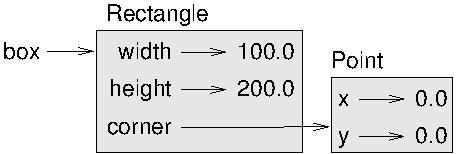
\includegraphics[scale=0.8]{../source/figs/rectangle.pdf}}
\caption{Object diagram.}
\label{fig.rectangle}
\end{figure}

Figure~\ref{fig.rectangle} shows the state of this object.
An object that is an attribute of another object is {\bf embedded}.

图~\ref{fig.rectangle} 展示了这个对象的状态。
一个对象作为另一个对象的属性叫做 {\em 嵌套} (embedded)。
\index{state diagram}  \index{diagram!state}
\index{object diagram}  \index{diagram!object}
\index{embedded object}  \index{object!embedded}


\section{Instances as return values  |  实例作为返回值}
\index{instance!as return value}  \index{return value}

Functions can return instances.  For example, \verb"find_center"
takes a {\tt Rectangle} as an argument and returns a {\tt Point}
that contains the coordinates of the center of the {\tt Rectangle}:

函数可以返回实例。 例如, \li{find_center} 接受一个 \li{Rectangle} 作为参数,
返回一个 \li{Point} ,代表了这个 \li{Rectangle} 的中心坐标:

\begin{lstlisting}
def find_center(rect):
    p = Point()
    p.x = rect.corner.x + rect.width/2
    p.y = rect.corner.y + rect.height/2
    return p
\end{lstlisting}

%
Here is an example that passes {\tt box} as an argument and assigns
the resulting Point to {\tt center}:

下面这个例子将 \li{box} 作为参数传递,然后将返回的 \li{Point} 赋值给 \li{center}:

\begin{lstlisting}
>>> center = find_center(box)
>>> print_point(center)
(50, 100)
\end{lstlisting}
%

\section{Objects are mutable  |  对象是可变的}
\index{object!mutable}  \index{mutability}

You can change the state of an object by making an assignment to one of
its attributes.  For example, to change the size of a rectangle
without changing its position, you can modify the values of {\tt
width} and {\tt height}:


你可以通过给一个对象的属性赋值来改变这个对象的状态。
例如,要改变一个矩形的大小而不改变它的位置,你可以修改 \li{width} 和 \li{height} 的值:

\begin{lstlisting}
box.width = box.width + 50
box.height = box.height + 100
\end{lstlisting}
%
You can also write functions that modify objects.  For example,
\verb"grow_rectangle" takes a Rectangle object and two numbers,
{\tt dwidth} and {\tt dheight}, and adds the numbers to the
width and height of the rectangle:

你也可以编写函数来修改对象。
例如,\li{grow_rectangle} 接受一个\li{Rectangle} 对象和两个数字,
\li{dwidth} 和\li{dheight} ,并将其加到矩形的宽度和高度上:

\begin{lstlisting}
def grow_rectangle(rect, dwidth, dheight):
    rect.width += dwidth
    rect.height += dheight
\end{lstlisting}
%
Here is an example that demonstrates the effect:

下面的例子展示了具体效果:

\begin{lstlisting}
>>> box.width, box.height
(150.0, 300.0)
>>> grow_rectangle(box, 50, 100)
>>> box.width, box.height
(200.0, 400.0)
\end{lstlisting}
%
Inside the function, {\tt rect} is an
alias for {\tt box}, so when the function modifies {\tt rect},
{\tt box} changes.

在函数内部, \li{rect} 是 \li{box} 的一个别名,
所以如果函数修改了 \li{rect} ,则 \li{box} 也随之改变。

As an exercise, write a function named \verb"move_rectangle" that takes
a Rectangle and two numbers named {\tt dx} and {\tt dy}.  It
should change the location of the rectangle by adding {\tt dx}
to the {\tt x} coordinate of {\tt corner} and adding {\tt dy}
to the {\tt y} coordinate of {\tt corner}.

我们做个练习,编写一个叫做 \li{move_rectangle} 的函数,接受一个 \li{Rectangle} 以及两个数字 \li{dx} 和 \li{dy}。  它把 \li{corner} 的 \li{x} 坐标加上 \li{dx},把 \li{corner} 的 \li{y} 坐标加上 \li{dy} ,从而改变矩形的位置。

\section{Copying  |  复制}
\label{copying}
\index{aliasing}

Aliasing can make a program difficult to read because changes
in one place might have unexpected effects in another place.
It is hard to keep track of all the variables that might refer
to a given object.

别名会降低程序的可读性,因为一个地方的变动可能对另一个地方造成预料之外的影响。
跟踪所有引用同一个对象的变量是非常困难的。
\index{copying objects}  \index{object!copying}
\index{copy module}  \index{module!copy}

Copying an object is often an alternative to aliasing.
The {\tt copy} module contains a function called {\tt copy} that
can duplicate any object:

通常用复制对象的方法取代为对象起别名。
\li{copy} 模块拥有一个叫做 \li{copy} 的函数,可以复制任何对象:

\begin{lstlisting}
>>> p1 = Point()
>>> p1.x = 3.0
>>> p1.y = 4.0

>>> import copy
>>> p2 = copy.copy(p1)
\end{lstlisting}

%
{\tt p1} and {\tt p2} contain the same data, but they are
not the same Point.

\li{p1} 和 \li{p2} 拥有相同的数据,但是它们并不是同一个 \li{Point} 对象。

\begin{lstlisting}
>>> print_point(p1)
(3, 4)
>>> print_point(p2)
(3, 4)
>>> p1 is p2
False
>>> p1 == p2
False
\end{lstlisting}

%
The {\tt is} operator indicates that {\tt p1} and {\tt p2} are not the
same object, which is what we expected.  But you might have expected
{\tt ==} to yield {\tt True} because these points contain the same
data.  In that case, you will be disappointed to learn that for
instances, the default behavior of the {\tt ==} operator is the same
as the {\tt is} operator; it checks object identity, not object
equivalence.  That's because for programmer-defined types, Python doesn't
know what should be considered equivalent.  At least, not yet.

正如我们预期的, \li{is} 运算符显示了 \li{p1} 和 \li{p2} 并非同一个对象。
不过你可能会认为 \li{==} 运算的结果应该是 \li{True} ,因为这两个点的数据是相同的。
然而结果并不如你想象的那样, \li{==} 运算符的默认行为和 \li{is} 运算符相同;
它检查对象的标识 (identity) 是否相同,而非对象的值是否相同。  因为 Python 并不知道什么样可以被认为相同。至少目前不知道。
\index{is operator}  \index{operator!is}
\index{identity}  \index{equivalence}

If you use {\tt copy.copy} to duplicate a Rectangle, you will find
that it copies the Rectangle object but not the embedded Point.
\index{embedded object!copying}

如果你使用 \li{copy.copy} 来复制一个 \li{Rectangle} ,
你会发现它仅仅复制了 \li{Rectangle} 对象,但没有复制嵌套的 \li{Point} 对象。

\begin{lstlisting}
>>> box2 = copy.copy(box)
>>> box2 is box
False
>>> box2.corner is box.corner
True
\end{lstlisting}

\begin{figure}
\centerline
{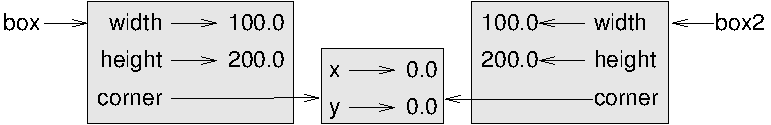
\includegraphics[scale=0.8]{../source/figs/rectangle2.pdf}}
\caption{Object diagram.}
\label{fig.rectangle2}
\end{figure}

Figure~\ref{fig.rectangle2} shows what the object diagram looks like.
\index{state diagram}  \index{diagram!state}
\index{object diagram}  \index{diagram!object}
This operation is called a {\bf shallow copy} because it copies the
object and any references it contains, but not the embedded objects.
\index{shallow copy}  \index{copy!shallow}

图~\ref{fig.rectangle2} 展示了相应的对象图。 这个操作叫做 {\em 浅复制} (shallow
copy) ,因为它仅复制了对象以及其包含的引用, 但未复制嵌套的对象。
\index{state diagram}  \index{diagram!state}
\index{object diagram}  \index{diagram!object}
\index{shallow copy}  \index{copy!shallow}

For most applications, this is not what you want.  In this example,
invoking \verb"grow_rectangle" on one of the Rectangles would not
affect the other, but invoking \verb"move_rectangle" on either would
affect both!  This behavior is confusing and error-prone.

对大多数应用来说,这并非是你想要的结果。
在这个例子中,对其中一个 \li{Rectangle} 对象调用 \li{grow_rectangle}并不会影响到另外一个, 然而当对任何一个 \li{Rectangle} 对象调用 \li{move_rectangle}的时候,两者都会被影响!这个行为很容易带来疑惑和错误。
\index{deep copy}  \index{copy!deep}

Fortunately, the {\tt copy} module provides a method named {\tt
deepcopy} that copies not only the object but also
the objects it refers to, and the objects {\em they} refer to,
and so on.  
You will not be surprised to learn that this operation is
called a {\bf deep copy}.

幸运的是, \li{copy} 模块拥有一个叫做 \li{deepcopy} 的方法,
它不仅可以复制一个对象,还可以复制这个对象所引用的对象,
甚至可以复制 {\bf 这个对象所引用的对象} 所引用的对象,等等。
没错!这个操作叫做 {\em 深复制} (deep copy) 。

\index{deepcopy function}  \index{function!deepcopy}

\begin{lstlisting}
>>> box3 = copy.deepcopy(box)
>>> box3 is box
False
>>> box3.corner is box.corner
False
\end{lstlisting}
%
{\tt box3} and {\tt box} are completely separate objects.

As an exercise, write a version of \verb"move_rectangle" that creates and
returns a new Rectangle instead of modifying the old one.

我们做个练习,编写另一个版本的 \li{move_rectangle} ,
函数创建并返回一个新的 \li{Rectangle} 对象而非修改原先的那个。

\section{Debugging  |  调试}
\label{hasattr}
\index{debugging}

When you start working with objects, you are likely to encounter
some new exceptions.  If you try to access an attribute
that doesn't exist, you get an {\tt AttributeError}:

当你开始学习对象的时候,你可能会遇到一些新的异常。
如果你访问一个不存在的属性,你会得到 \li{Attributeerror} 的错误提示:

\index{exception!AttributeError}  \index{AttributeError}

\begin{lstlisting}
>>> p = Point()
>>> p.x = 3
>>> p.y = 4
>>> p.z
AttributeError: Point instance has no attribute 'z'
\end{lstlisting}

%
If you are not sure what type an object is, you can ask:

如果你不确定一个对象的类型,你可以询问:

\index{type function}  \index{function!type}

\begin{lstlisting}
>>> type(p)
<class '__main__.Point'>
\end{lstlisting}

%
You can also use {\tt isinstance} to check whether an object
is an instance of a class:

你也可以用 \li{isinstance} 来检查某个对象是不是某个类的实例。

\index{isinstance function}  \index{function!isinstance}

\begin{lstlisting}
>>> isinstance(p, Point)
True
\end{lstlisting}

%
If you are not sure whether an object has a particular attribute,
you can use the built-in function {\tt hasattr}:

如果你不确定一个对象是否拥有某个属性, 你可以使用内置函数 \li{hasattr} 检查:
\index{hasattr function}  \index{function!hasattr}

\begin{lstlisting}
>>> hasattr(p, 'x')
True
>>> hasattr(p, 'z')
False
\end{lstlisting}
%
The first argument can be any object; the second argument is a {\em
string} that contains the name of the attribute.

第一个参数可以是任何对象;
第二个参数是一个 {\em 字符串} ,代表了某个属性的名字。

\index{attribute}

You can also use a {\tt try} statement to see if the object has the
attributes you need:

你也可以使用 \li{try} 语句来检查某个对象是不是有你需要的属性:

\index{try statement}  \index{statement!try}

\begin{lstlisting}
try:
    x = p.x
except AttributeError:
    x = 0
\end{lstlisting}

This approach can make it easier to write functions that work with
different types; more on that topic is
coming up in Section~\ref{polymorphism}.

这个方法可以让你更容易编写出可以适应多种数据结构的函数。你可以在 \ref{polymorphism}~节 查看更多内容。


\section{Glossary  |  术语表}

\begin{description}

\item[class:] A programmer-defined type.  A class definition creates a new
class object.

\item[类(class):] 一种程序员自定义的类型。类定义创建了一个新的类对象。
\index{class}  \index{programmer-defined type}  \index{type!programmer-defined}

\item[class object:] An object that contains information about a
programmer-defined type.  The class object can be used to create instances
of the type.

\item[类对象(class object):]包含程序员自定义类型的细节信息的对象。类对象可以被用于创建该类型的实例。

\index{class object}  \index{object!class}

\item[instance:] An object that belongs to a class.

\item[实例(instance):] 属于某个类的对象。
\index{instance}

\item[instantiate:] To create a new object.

\item[实例化(instantiate):] 创建新的对象。
\index{instantiate}

\item[attribute:] One of the named values associated with an object.

\item[属性(attribute):] 和某个对象相关联的有命名的值。
\index{attribute!instance}  \index{instance attribute}

\item[embedded object:] An object that is stored as an attribute
of another object.

\item[嵌套对象(embedded object):] 作为另一个对象的属性存储的对象。
\index{embedded object}  \index{object!embedded}

\item[shallow copy:] To copy the contents of an object, including
any references to embedded objects;
implemented by the {\tt copy} function in the {\tt copy} module.

\item[浅复制(shallow copy):]在复制对象内容的时候,只包含嵌套对象的引用,通过 \li{copy} 模块的 \li{copy} 函数实现。
\index{shallow copy}

\item[deep copy:] To copy the contents of an object as well as any
embedded objects, and any objects embedded in them, and so on;
implemented by the {\tt deepcopy} function in the {\tt copy} module.

\item[深复制(deep copy):]在复制对象内容的时候,既复制对象属性,也复制所有嵌套对象及其中的所有嵌套对象,由 \li{copy} 模块的 \li{deepcopy} 函数实现。
\index{deep copy}

\item[object diagram:] A diagram that shows objects, their
attributes, and the values of the attributes.

\item[对象图(object diagram):] 展示对象及其属性和属性值的图。
\index{object diagram}  \index{diagram!object}

\end{description}


\section{Exercises  |  练习}

\begin{exercise}

Write a definition for a class named {\tt Circle} with attributes
{\tt center} and {\tt radius}, where {\tt center} is a Point object
and radius is a number.

定义一个叫做 \li{Circle} 类,类的属性是圆心( \li{center} ) 和半径( \li{radius} ),其中,圆心( \li{center}) 是一个 \li{Point} 类,而半径( \li{radius})是一个数字。

Instantiate a Circle object that represents a circle with its center
at $(150, 100)$ and radius 75.

实例化一个圆心(center)为 $(150, 100)$ ,半径(radius)为 75 的 $Circle$ 对象。

Write a function named \verb"point_in_circle" that takes a Circle and
a Point and returns True if the Point lies in or on the boundary of
the circle.

编写一个名称为 \li{point_in_circle} 的函数,该函数可以接受一个圆类( \li{Circle})对象和点类 ( \li{Point} )对象,然后判断该点是否在圆内。 在圆内则返回 \li{True} 。

Write a function named \verb"rect_in_circle" that takes a Circle and a
Rectangle and returns True if the Rectangle lies entirely in or on the boundary
of the circle.

编写一个名称为 \li{rect_in_circle} 的函数,该函数接受一个圆类( \li{Circle})对象和矩形( \li{Rectangle})对象,如果该矩形是否完全在圆内或者在圆上则返回 \li{True} 。

Write a function named \verb"rect_circle_overlap" that takes a Circle
and a Rectangle and returns True if any of the corners of the Rectangle fall
inside the circle.  Or as a more challenging version, return True if
any part of the Rectangle falls inside the circle.

编写一个名为 \li{rect_circle_overlap} 函数,该函数接受一个圆类对象和一个矩形类对象,如果矩形有任意一个角落在圆内则返回 \li{True} 。 或者写一个更具有挑战性的版本,如果该矩形有任何部分落在圆内返回 \li{True} 。

Solution: \url{http://thinkpython2.com/code/Circle.py}.

\href{http://thinkpython2.com/code/Circle.py}{参考答案}

\end{exercise}

\begin{exercise}

Write a function called \verb"draw_rect" that takes a Turtle object
and a Rectangle and uses the Turtle to draw the Rectangle.  See
Chapter~\ref{turtlechap} for examples using Turtle objects.

编写一个名为 \li{draw_rect} 的函数,该函数接受一个 \li{Turtle} 对象和一个 \li{Rectangle} 对象,使用 \li{Turtle} 画出该矩形。参考 \ref{turtlechap} 章中使用 \li{Turtle} 的示例。

Write a function called \verb"draw_circle" that takes a Turtle and
a Circle and draws the Circle.

编写一个名为 \li{draw_circle} 的函数,该函数接受一个 \li{Turtle} 对象和 \li{Circle} 对象,并画出该圆。

Solution: \url{http://thinkpython2.com/code/draw.py}.

\href{http://thinkpython2.com/code/draw.py}{参考答案}

\end{exercise}